\begin{abstract}
  This paper addresses scene understanding in the context of a moving
  camera, integrating semantic reasoning ideas from monocular vision
  with 3D information available through structure--from--motion. We
  combine geometric and photometric cues in a Bayesian framework,
  building on recent successes leveraging the indoor Manhattan
  assumption in monocular vision. We focus on indoor environments and
  show how to extract key boundaries while ignoring clutter and
  decorations. To achieve this we present a graphical model that
  relates photometric cues learned from labeled data, stereo
  photo--consistency across multiple views, and depth cues derived
  from structure--from--motion point clouds. We show how to solve MAP
  inference using dynamic programming, allowing exact, global
  inference in $\sim$$100$ ms (in addition to feature computation of
  under one second) without using specialized hardware. Experiments
  show our system out--performing the state--of--the--art.
\end{abstract}

\section{Introduction}
Over the past decade, computer vision researchers working with
monocular images have pursued substantially different research
agendas to those working with multiple views. The focus for
monocular images has increasingly been to infer high--level facts
about the world, such as the locations of and interactions between
objects, semantic scene categories, and the spatial layout of the
environment. In contrast, much of the work concerning multiple views
has focused on reconstructing metric scene structure and camera poses
using techniques such as structure--from--motion, stereo, and
multiple--view stereo.

In this paper we leverage multiple view geometry for image
understanding purposes. We assume a moving camera with a
structure--from--motion system estimating its trajectory, and show how
to infer semantically meaningful models of the environment. We focus
on the \textit{indoor Manhattan representation}\cite{Lee09,FlintECCV10}, in which the world is
modeled in terms of floor, wall, and ceiling surfaces. This
representation captures many semantically meaningful aspects of the
environment, including (i) scale: the distance from floor to ceiling
suggests a scale for distances in the environment; (ii) boundaries:
walls constrain movement in the environment and suggest locations for
doors, windows, and other objects; (iii) gravity: the orientation of
the ground plane implies the direction in which gravity operates,
which constrains the arrangement of objects resting upon one another;
and (iv) shape: the organisation of walls in an environment suggests
a functional category (such as ``kitchen'' or ``office'').


\begin{figure}[tb]%
  \centering
  %\begin{tabular}{c}
    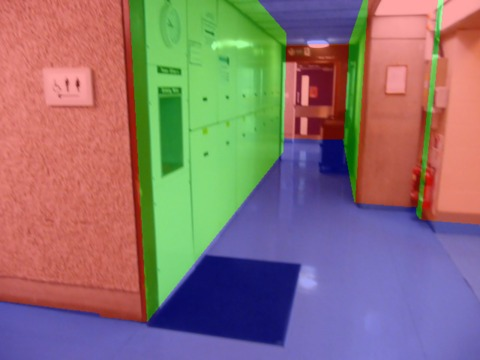
\includegraphics[width=0.2\textwidth]{figures/firstpage/lab_foyer2_frame041_dp.jpg}
    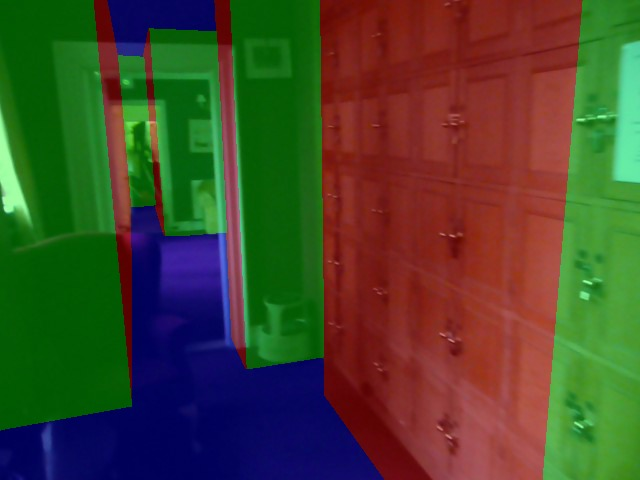
\includegraphics[width=0.2\textwidth]{figures/firstpage/exeter_mcr1_frame032_dp.jpg}
  %\end{tabular}
  \caption{Automatic reconstructions from our system.}
  %\label{fig:results-pics-top}
    \vspace{-5mm}
  \label{fig:firstpage}
\end{figure}

Indoor Manhattan models are useful because they capture these
properties explicitly, whereas to extract such properties from a dense
polygonal mesh would require additional non--trivial inference after
reconstruction. Our approach infers semantic properties of the scene
directly from multiple--view data, without an intermediate dense
reconstruction step. This makes sense if, as in our case, the semantic
properties constitute the ultimate goal of the system. Of course, if a
photo--realistic reconstruction is itself the end goal then our
approach is not suitable.

We build on recent work highlighting the efficacy of the indoor
Manhattan representation for single view reconstruction
\cite{Lee09,FlintECCV10}. Previous work employed a set of
heuristics as a cost function and was limited to monocular images. We
give a fully Bayesian account in which information from image
features, stereo, and 3D point clouds is integrated into a single MAP
optimization, and we learn all parameters from labeled examples. We
show that MAP inference in our model can be solved exactly and
efficiently ($\sim$$100$ ms per frame) using a generalization of the
dynamic programming algorithm of
\cite{FlintECCV10}.

%% Our work extends their approach to allow joint inference across
%% multiple views as well as to incorporate range data alongside
%% photometric cues. This involves a significant generalization of
%% their algorithm since neither of these new modalities are
%% representable using their pixel--wise cost function. We therefore
%% generalize their approach to a payoff--based formulation permitting
%% more general costs. We also show that in this new formulation one
%% of the state variables involved in their optimisation is
%% unecessary; its removal corresponds to eliminating an entire
%% dimension from the search and results in an order of magnitude
%% efficiency improvement.

%XXX Un-comment next para?
%When comparing our approach to previous work we propose that in
%addition to measuring geometric accuracy, the \textit{size} of
%alternative representations should also be compared, since models that
%capture key properties of the environment using fewer representational
%bits must have done a better job of filtering salient information
%from sensor data. This is in line with the relationship between the
%ability of an algorithm to compress data and its ability to make
%predictions (cite Hutter).

The remainder of this paper is organised as follows. Section two
places our contribution in context with related work. We introduce our
model in section three, then we describe inference in section four and
learning in section five. We give experimental results in section six,
followed by concluding remarks in section seven.

\begin{figure}[tb]%
  \centering
  \label{fig:ideal-models}
  \begin{tabular}{ccc}
    %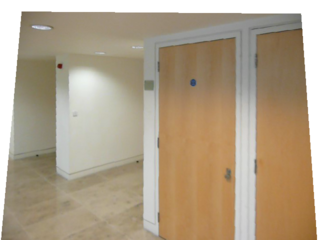
\includegraphics[width=0.12\textwidth]{figures/true_models/lab_ground1_010_rect.png} &
    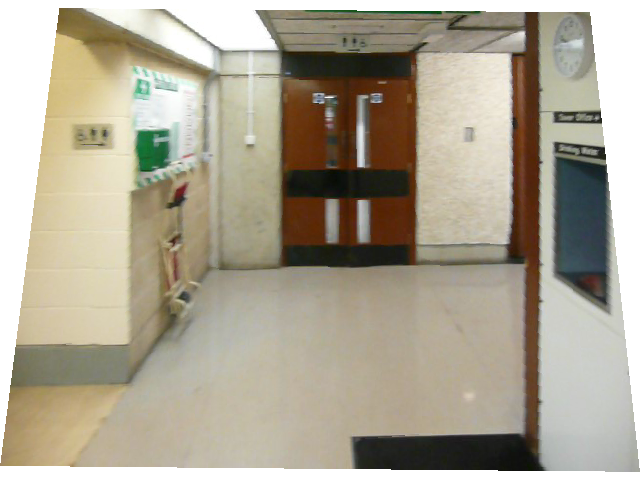
\includegraphics[width=0.12\textwidth]{figures/true_models/lab_foyer1_010_rect.png} &
    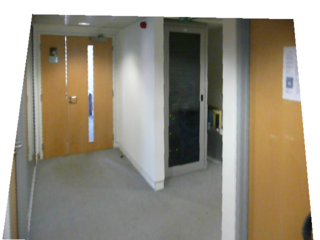
\includegraphics[width=0.12\textwidth]{figures/true_models/lab_kitchen_030_rect.png} &
    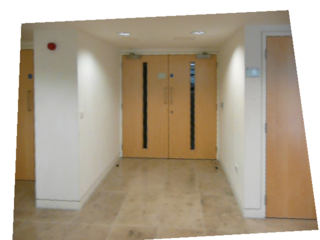
\includegraphics[width=0.12\textwidth]{figures/true_models/lab_ground1_030_rect.png} \\
    %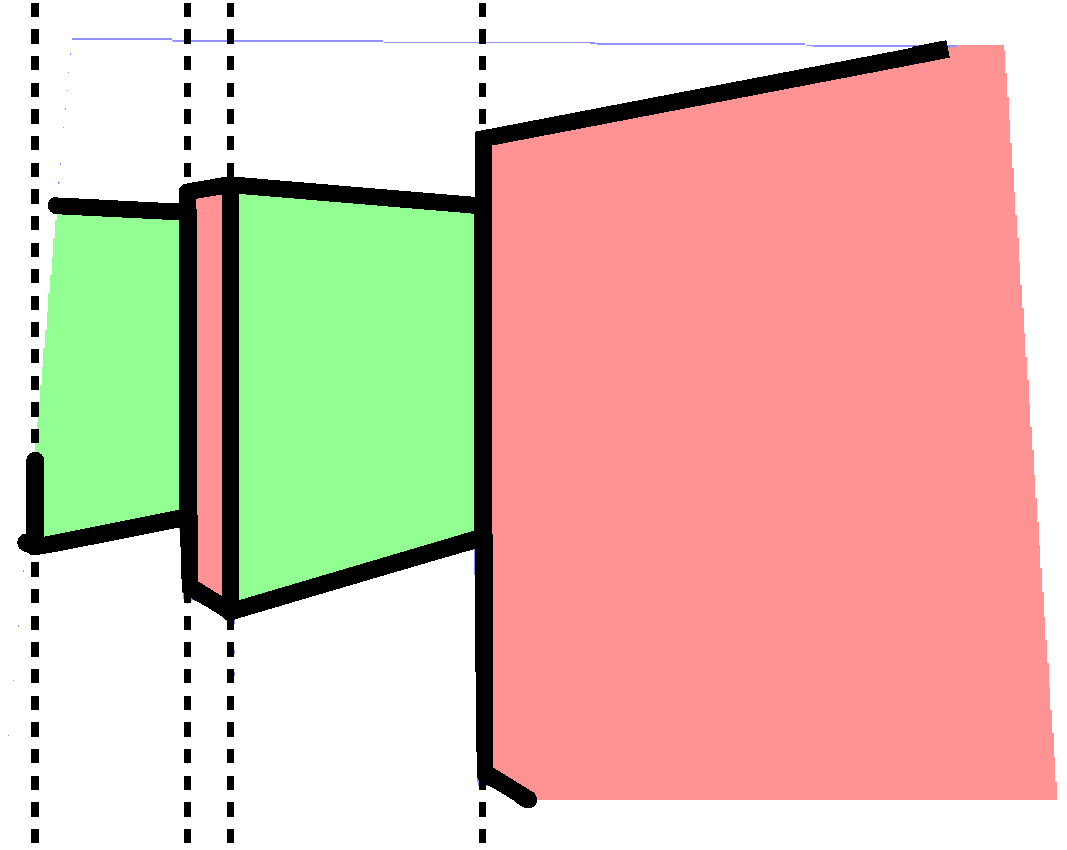
\includegraphics[width=0.12\textwidth]{figures/true_models/lab_ground1_010} &
    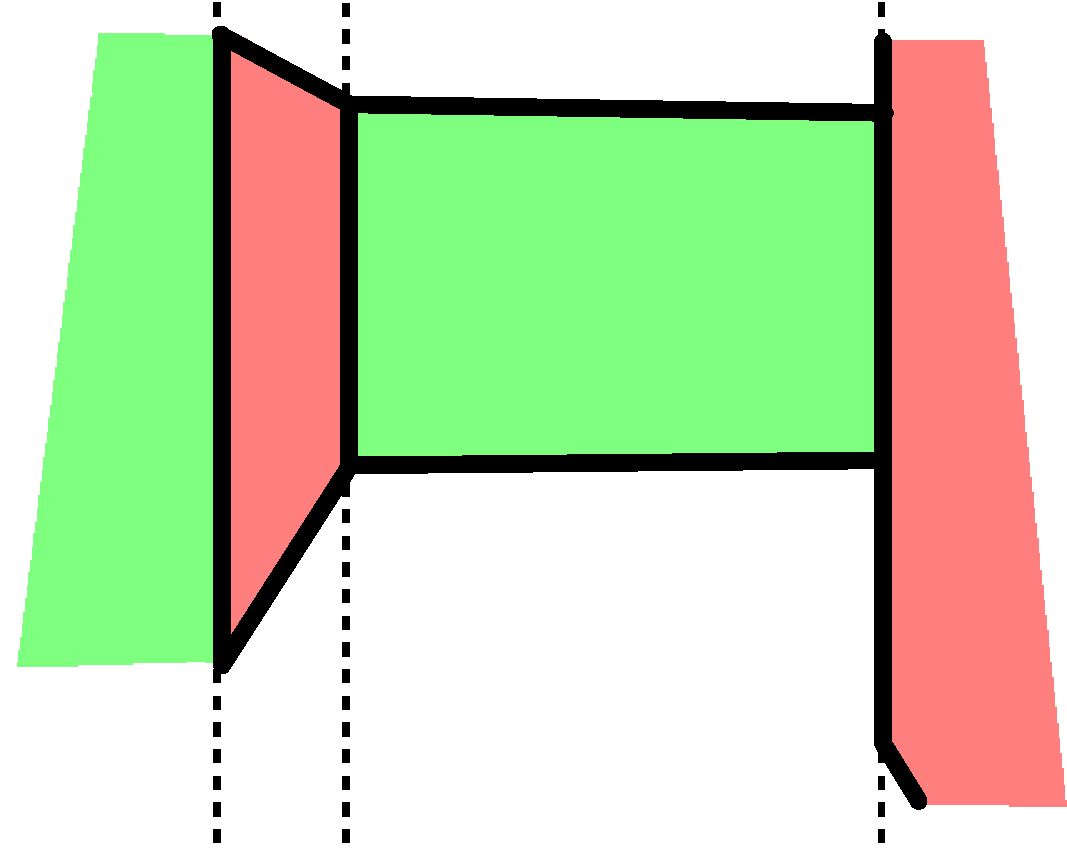
\includegraphics[width=0.12\textwidth]{figures/true_models/lab_foyer1_010} &
    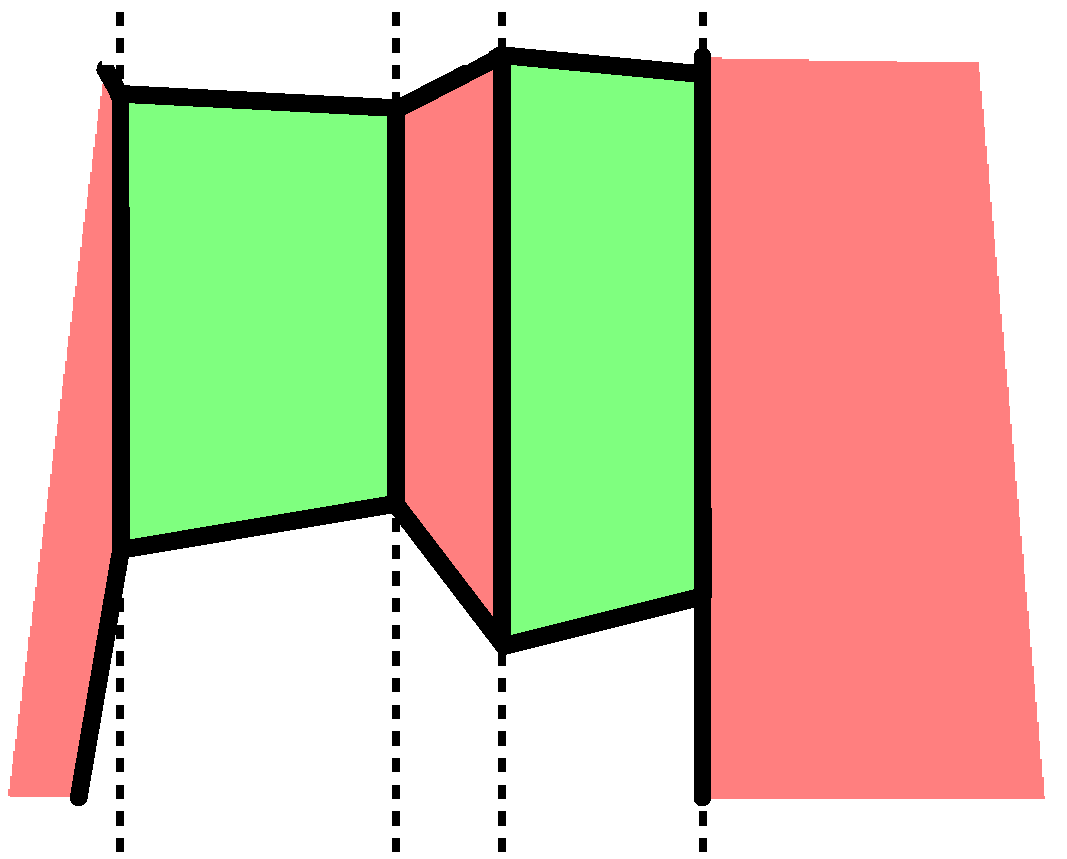
\includegraphics[width=0.12\textwidth]{figures/true_models/lab_kitchen_030} &
    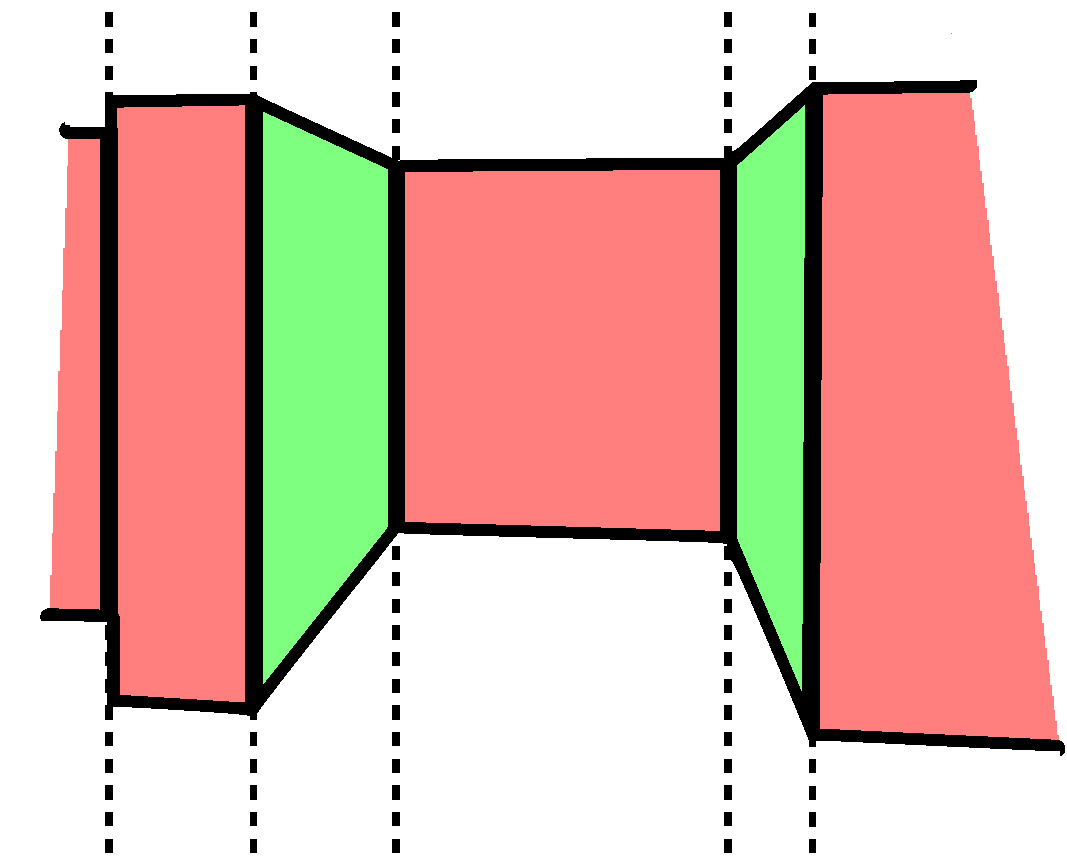
\includegraphics[width=0.12\textwidth]{figures/true_models/lab_ground1_030}
  \end{tabular}
  \hspace{0.2cm}
  \caption{Three input images and the indoor Manhattan models we
    seek. Notice how each image column intersects exactly one wall.}
\end{figure}

\section{Background}
The Manhattan world assumption was introduced by Coughlan and
Yuille\cite{Coughlan99} over a decade ago and has seen increasing
attention in the computer vision literature over past years
\cite{Coughlan99,Zhang02,Lee09,Furukawa09,FlintECCV10}. Furukawa
\etal \cite{Furukawa09} proposed a Manhattan--world stereo algorithm
based on graph cuts. While their approach is concerned with dense
photo--realistic reconstructions, ours is intended to capture semantic
properties of the scene using a concise representation. The output of
their approach --- a polygonal mesh --- has no immediate semantic
interpretation, whereas our models, though less detailed, come
packaged with a direct interpretation. A by--product is efficiency: we
count computation time in hundreds of milliseconds, where as
Furukawa \etal report waiting more than an hour.

Another approach to interpreting Manhattan worlds is to model scenes
as a union of cuboids. This approach has a long history beginning with
Roberts' 1965 thesis \cite{Roberts65}, and has recently been revisited
using modern probabilistic techniques \cite{Gupta10,Vanegas10}.

Lee \etal \cite{Lee09} first proposed indoor Manhattan models (a
sub--class of general Manhattan models) for monocular
reconstructions. They used a branch--and--bound algorithm together
with a line--sweep heuristic for approximate inference. Flint \etal
\cite{FlintECCV10} employed a similar model but showed a
dynamic programming algorithm that performed exact inference in
polynomial time. In earlier work \cite{FlintCVPR10} Flint \etal also
demonstrated Manhattan reconstructions integrated with a SLAM system,
but this work inferred models from single frames and then extrapolated
these forward in time. In contrast, our work incorporates both
multiple view geometry and 3D points directly into a joint inference
procedure. We also learn parameters in a Bayesian framework, where as
neither Lee nor Flint utilized training data in any form.

Felzenszwalb and Veksler \cite{Felzenszwalb10} posed the
reconstruction problem in terms of energy minimization, which they
showed could be solved using dynamic programming, while Barinova \etal
\cite{Barinova08} modeled outdoor scenes using a CRF. However, these
approaches do not permit strong geometric constraints and so cannot be
extended to multiple views.

Semantic scene understanding has, broadly speaking, seen less
attention within the multiple view community. The CamVid
\cite{Brostow08} database of outdoor videos with semantic
segmentations is an important and encouraging exception. Brostow \etal
\cite{Brostow08} showed that simple structure--from--motion cues lead
to pleasing segmentations. Sturgess \etal \cite{Sturgess09} extended
this approach to a CRF framework. We compare our method with this
approach in \sectref{results}.

%XXX Do we need to cite work on object/action recognition, point cloud
%labelling?
% Object/action recognition
%   Leibe et al CVPR 2007 (best paper) SfM+object detection
%   Dala et al, ECCV 2006 HOG+flow
% Point labelling
%   Golovinskiy et al, ICCV 2009,  http://www.cs.princeton.edu/~funk/iccv09.pdf
%   Munoz et al, 2009 tech report: http://repository.cmu.edu/cgi/viewcontent.cgi?article=1329&context=robotics
% Our approach doesn't require 3D points at all, but can work with
% sparse OR dense points if available, and integrates with stereo +
% photometric features.

%XXX: The ECCV(?) paper on using manhattan + non-manhattan surfaces for
%reconstruction.

\section{Proposed Model}
\label{sect:model}

\begin{figure}[tb]%
  \centering
  \label{fig:corner-types}
  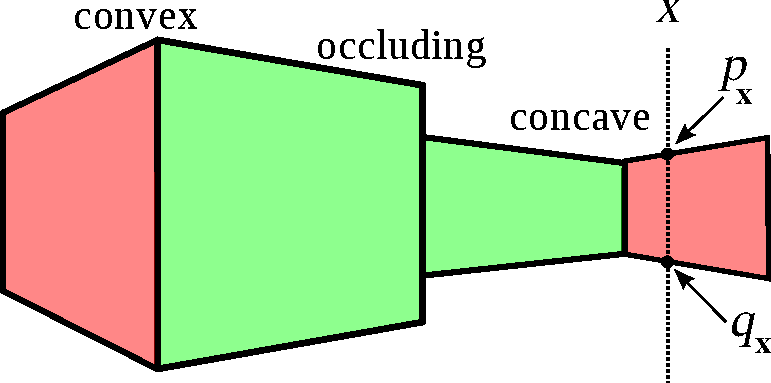
\includegraphics[width=0.3\textwidth]{figures/corner-types}
  \hspace{0.1cm}
  \caption{Each corner in an indoor Manhattan environment can be
    categorized as concave, convex, or occluding. Each vertical line
    intersects exactly one wall segment, the top and bottom of which
    we denote $\PfAtX$ and $\PcAtX$ respectively.}
\end{figure}

In this section we describe the indoor Manhattan model. We consider
three sensor modalities: monocular image features, stereo features,
and 3D point clouds. For each we present a generative model relating
observed features to the Manhattan scene structure, which we denote
$\Model$. For each sensor modality we show that MAP inference can be
reduced to maximization over a payoff function
$\PixelPayoff(x,y)$. This allows us to present a unified dynamic
programming solution in \sectref{inference}, which efficiently solves
MAP inference for all three sensor modalities.

%In this section we describe indoor Manhattan models and pose inference
%within this class as maximization of a payoff function that decomposes
%over image columns.\footnote{Only the marginal likelihoods (or unary
%potentials in the language of energy functions) decompose in this
%way. Our prior permits strong coupling across widely separated image
%columns.} We will then present generative models for photometric,
%multiple--view, and 3D features that give rise to MAP formulae that
%can be expressed in precisely this form. This will allow us
%in \sectref{inference} to provide a concise dynamic programming
%solution in the abstract setting of payoff matrices.

General Manhattan environments have structural surfaces oriented in
three cardinal orientations. \textit{Indoor} Manhattan environments
are a special case that consist of a floor plane, a parallel ceiling
plane, and a set of vertical walls extending between them. Each wall
extends all the way from the floor to ceiling, and walls meet at
vertical edges. We always consider environments observed from a camera
located between the floor and ceiling. Since each wall extends from
floor to ceiling, indoor Manhattan environments always project
as a linear chain of walls in the image, as shown in
\figref{ideal-models}. Further, the edges at which adjacent walls meet
can be categorized as concave, convex, or occluding, as illustrated in
\figref{corner-types} and discussed further in \cite{Lee09}.

We assume that vanishing points for the three Manhattan directions are
given. We use the vanishing point detector described by Zhang \etal
\cite{Zhang02} in the monocular setting and that of \cite{FlintCVPR10} in
the multiple view setting. It will greatly simplify the remainder of
this paper if we can assume that vertical lines in the world appear
vertical in the image. To this end we apply the simple rectification
procedure of \cite{FlintCVPR10}.
%\footnote{Note that we could avoid the
%  warping artifacts introduced by this operation and instead carry
%  through geometric calculations assuming a general camera pose, but
%  this would make the remainder of this paper much harder to follow.}

We now describe our parametrization for indoor Manhattan models. Let
the image dimensions be $\Width \times \Height$. Following
rectification, the vertical seams at which adjacent walls meet project
to vertical lines, so each image column intersects exactly one wall
segment. Let the top and bottom of the wall in column $x$ be
$\PfAtX=(x,\YfAtX)$ and $\PcAtX=(x,\YcAtX)$ respectively (depicted in
\figref{corner-types}). Since each $\PfAtX$ lies on the floor plane
and each $\PcAtX$ lies on the ceiling plane, we have
\begin{equation}
\label{eq:manhattan-homology}
  \PfAtX = \Hcf \PcAtX ~.
\end{equation}
where $\Hcf$ is a planar homology \cite{Criminisi01}. We show how to
recover $\Hcf$ in \sectref{floorceil}. Once $\Hcf$ is known, any
indoor Manhattan model is fully described by the values $\{\YfAtX\}$,
leading to the simple parametrization,
\begin{equation}
  \Model = \{ \YfAtX \}_{x=1}^{\Width} ~.
\end{equation}
We query this parametrization as follows. To check whether a pixel
$(x_0,y_0)$ lies on a vertical or horizontal surface we simply need to
check whether $y_0$ is between $\YfAtXX$ and $\YcAtXX$. If we know the
3D position of the floor and ceiling planes then we can recover the
depth of every pixel as follows. If the pixel lies on the floor or
ceiling then we simply back--project a ray onto the corresponding
plane. If not, we back--project onto the vertical plane defining the
wall at that column (the depth of which we can recover from
$\YfAtXX$). Note in particular that the orientation and depth of a
pixel can be recovered from just the floor/wall intersection in its
column; this will be important in later sections.

We now turn to the optimization framework that each subsequent section
will feed into. Let $\{c_i\}$ index the columns at which neighbouring
walls meet in $\Model$. We define the payoff for $\Model$ as
\begin{equation}
  \label{eq:payoffs}
  \ModelPayoff(\Model) = 
  \sum_{x=1}^{\Width} \PixelPayoff(x,\YfAtX) -
  \sum_i \CornerPenalty(c_i) \,
\end{equation}
where the payoff matrix $\PixelPayoff$ assigns payoffs for models with
floor/wall intersections that pass through each pixel, and
$\CornerPenalty$ is a per--corner regulariser which penalizes complex
models. Note that the value of $\PixelPayoff(x,y)$ is \textit{not}
restricted to dependence on pixel $(x,y)$, nor even to a local region
about that pixel; indeed, the payoff functions described in the
following sections incorporate image evidence from widely separated
image regions.

\subsection{Monocular features}

\begin{figure}[tb]
  \centering
  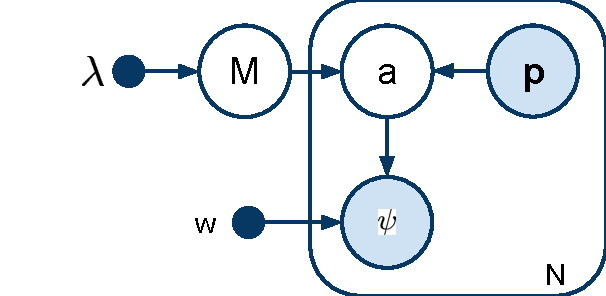
\includegraphics[width=0.35\textwidth]{figures/monocular-gm}
  \caption{The graphical model relating building structures $M$ to
    monocular image features $\Feature$. $\Pixel=(x,y)$ is a
    pixel location and $a$ is the orientation predicted (deterministically) by
    $\Model$ at $\Pixel$.}
  \label{fig:monocular-gm}
\end{figure}

To infer indoor Manhattan models from monocular images we assume the
graphical model shown in \figref{monocular-gm}. We turn first to the
prior $P(\Model~|~\Penalties)$. For a model with $n_1$ concave
corners, $n_2$ convex corners, and $n_3$ occluding corners
(\cf \figref{corner-types}), our prior on models is
\begin{eqnarray}
  \label{eq:model-prior}
  P(\Model ~|~ \Penalties) &=& \frac{1}{Z} 
    {\PenaltyConc}^{n_1} {\PenaltyConv}^{n_2} {\PenaltyOccl}^{n_3}
  % \\
  %Z &=& \sum_{n_c,n_n,n_o} P(\Model ~|~ \Penalties) \\
  %Z&=& \frac{1}{(1-\PenaltyConc)(1-\PenaltyConv)(1-\PenaltyOccl)}~,
\end{eqnarray}
which corresponds to a fixed probability for ``events'' corresponding
to each type of corner and penalizes models for additional
complexity. $Z$ is a normalizing constant.

Our model includes hidden orientation variables
$\Orient_i\in\{1,2,3\}$ for each pixel, with values corresponding to
the three Manhattan orientations (shown as red, green, and blue
regions in \figref{ideal-models}). As described in \sectref{model},
$\Orient$ is deterministic given the model $\Model$. We assume a
linear likelihood for pixel features $\Feature$,
\begin{equation}
\label{eq:feature-likelihood}
  P(\Feature ~|~ \Orient) = \frac{{\PixelModel_\Orient}^T\Feature}
  {\sum_j{\PixelModel_\Orient}^T\Feature_j} ~.
\end{equation}

We now derive MAP inference. The posterior on $\Model$ is
\begin{align}
  \label{eq:mono-post}
  P(\Model ~|~ \Features) = {} &
  \eta P(\Model) \prod_i P(\Feature_i ~|~ \Orient_i^*)
\end{align}
where $\Orient_i^*$ is the orientation deterministically predicted by
model $\Model$ at pixel $\Pixel_i$ and $\eta$ is a normalizing
constant. We have omitted $P(\Orient_i~|~\Model)$ since it equals
1 for $\Orient_i^*$ and 0 otherwise. Taking logarithms,
\begin{align}
  \label{eq:mono-logpost}
  \begin{split}
    \log P(\Model ~|~ \Features) = {} &
    n_1 \PenaltyConc' + n_2 \PenaltyConv' + n_3 \PenaltyOccl'
    \\    
    & + \sum_i \log P(\Feature_i ~|~ \Orient_i^*) + k
  \end{split}
\end{align}
where $\PenaltyOccl'=\log \PenaltyOccl$ and similarly for the other
penalties, and $k$ corresponds to the normalizing denominators in
\eqnref{mono-post} and \eqnref{model-prior}, which we henceforth drop
since it makes no difference to the optimization to come. We can now
put \eqnref{mono-logpost} into payoff form \eqnref{payoffs} by writing
\begin{equation}
  \label{eq:mono-payoffs}
  \begin{split}
    \MonoPayoff(x,\ModelAtX) =&
    \sum_{y'} \log P(\Feature_i ~|~ \Orient_i^*) \\
    \MonoCornerPenalty(c) =& -\lambda_c
  \end{split}
\end{equation}
where $\lambda_c$ is one of $\PenaltyConc$, $\PenaltyConv$, or
$\PenaltyOccl$ according to the category of corner $c$. We show how to
maximize payoffs of this form in \sectref{inference}, which will allow
us to solve MAP inference.

\subsection{Multiple view features}
\begin{figure}[tb]
  \centering 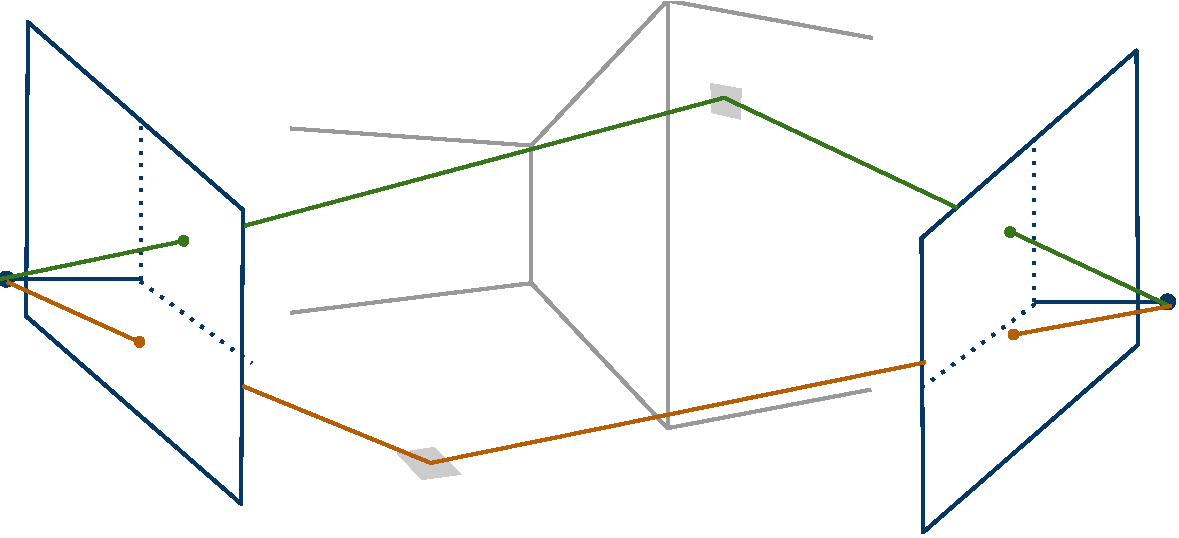
\includegraphics[width=0.4\textwidth]{figures/backproject}
  \caption{Pixel correspondences across multiple views are computed by
    back--projection onto the model $\Model$ followed by re--projection into
    auxiliary views.}
  \label{fig:backproject}
\end{figure}
We now formulate the payoff function $\StereoPayoff$ for the case that
multiple views of the scene are available. We assume one base frame
$I_0$ and $M$ auxiliary frames $I_1,\ldots,I_M$. We assume that poses
are given for each camera, as output for example by a
structure--from--motion system, and that cameras are calibrated. We
normalize images intensities to zero mean and unit variance.

Intuitively, we treat inference in this settings as follows. We
consider models $\Model$ in terms of their projection into $I_0$. We
explained in \sectref{model} that models parametrized in image
coordinates specify unique 3D models. Any hypothesized model can
therefore be re--projected into auxiliary frames, giving pixel--wise
correspondences between frames as shown in \figref{backproject}. From
this we compute a photo--consistency measure $\pc(\cdot)$, which
provides the likelihood $P(\StereoData ~|~ \Model)$. The prior remains
as in \eqnref{model-prior}.

Optimizing over photo--consistency has been standard in the stereo
literature for several decades \cite{Scharstein01}; our contribution
is to show that (i) in the particular case of indoor Manhattan models,
photo--consistency can be expressed as a payoff matrix; (ii) that we
can therefore perform efficient and exact global optimization; and
(iii) that this fits naturally within a Bayesian framework alongside
monocular and 3D features.

% SPACE: remove para below
Our approach could also be cast as solving the general stereo problem
where in place of priors based on various pixel--wise norms, our prior
assigns zero probability to all non--indoor--Manhattan
reconstructions.

Let $\reproj_k(\Pixel;\Model)$ be the re--projection of pixel $\Pixel$
from the base frame $I_0$ into auxiliary frame $I_k$ via model
$\Model$. Then
\begin{equation}
  \label{eq:stereo-likelihood}
  \log P(\StereoData ~|~ \Model) = 
   \sum_{\Pixel\in I_o} \sum_{k=1}^M
  \pc(\Pixel,\reproj_k(\Pixel,\Model)) ~,
\end{equation}
where in our experiments $\pc(\Pixel,\Qixel)$ is the sum of squared
differences between pixels $\Pixel$ and $\Qixel$. 

%Equation
%\eqnref{stereo-likelihood} could be derived from a graphical model
%assuming a joint Gaussian relationship across correspondences, but we
%have skipped this because it is standard in the literature
%\cite{Scharstein01}.

We explained in \sectref{model} that the depth of each pixel can be
recovered from the location of the floor/wall intersection $\ModelAtX$
in column $x$. Hence we can replace $\reproj_k(\Pixel;\Model)$ with
$\reproj_k(\Pixel;\ModelAtX)$ and write
\begin{equation}
  \label{eq:stereo-payoffs}
  \StereoPayoff(x,y_x) = 
    \sum_{y=1}^{\Height} \sum_{k=1}^M
      \pc(\Pixel,\reproj_k(\Pixel,y_x)) ~,
\end{equation}
where $\Pixel=(x,y)$. To see this, substitute \eqnref{stereo-payoffs}
into \eqnref{payoffs} and observe that the result is
precisely \eqnref{stereo-likelihood}.

Note that the column--wise decomposition \eqnref{stereo-payoffs}
neither commits us to optimizing over columns independently, nor to
ignoring interactions between columns. Such interactions come into
effect when we optimize over the full payoff matrix
in \sectref{inference}, and our results will show that widely
separated image regions often interact strongly. The derivations
in this section follow deductively from the indoor Manhattan
assumption; the only approximation is the following.

\textbf{Occlusions}. We have ignored self--occlusions in
\eqnref{stereo-likelihood}. For short baselines (such as frames
sampled over a few seconds from a moving camera), this is
unproblematic since indoor environments tend to be mostly convex from
any single point of view. Even in highly non--convex environments our
system achieves excellent results by integrating 3D and monocular
features, and enforcing strong global consistency, as will be shown in
\sectref{results}.

%\subsubsection{Extension: using orientation information}

%\subsubsection{EM for Occlusion Resolution}

\subsection{3D features}
\begin{figure}[tb]
  \centering
  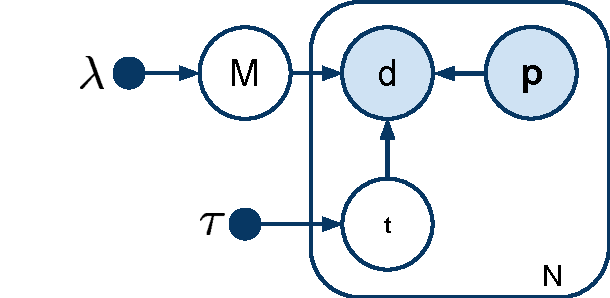
\includegraphics[width=0.35\textwidth]{figures/3d-gm}
  \caption{The graphical model relating indoor Manhattan models to 3D
    points. The hidden variable $t$ indicates whether the point is
    inside, outside, or coincident with the model.}
  \label{fig:3d-gm}
\end{figure}

In this section we explore the context in which a 3D point cloud is
available during inference. The point clouds generated by
structure--from--motion systems are typically too sparse for direct
reconstruction, but can provide useful cues alongside monocular and
stereo data.

\begin{figure}[tb]
  \centering 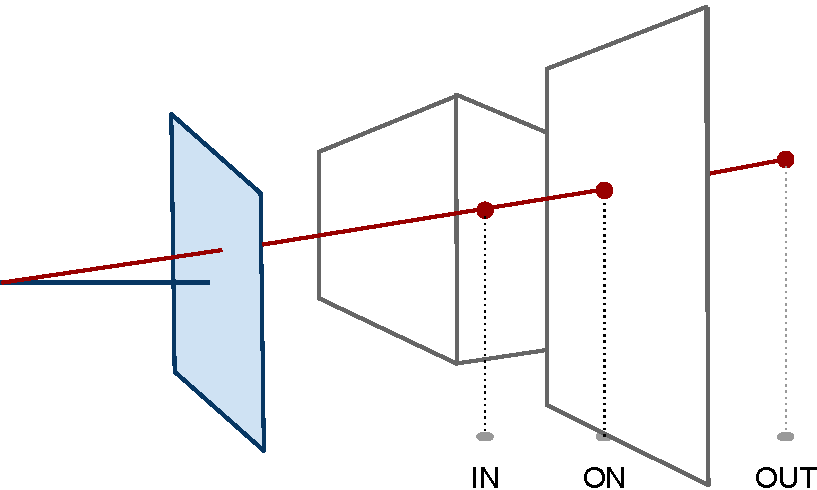
\includegraphics[width=0.3\textwidth]{figures/point-projs}
  \caption{Depth measurements $d_i$ might be generated by a surface in
    our model (represented by $t_i=\ON$) or by an object inside or
    outside the environment (in which case $t_i=\IN,\OUT$
    respectively).}
  \label{fig:point-projs}
\end{figure}


%For each pixel $\Pixel_i$ a depth measurement $d_i$ is made. The
%relationship between $d$ and the model $M$ is determined by a hidden
%variable $t\in\{\textsf{IN},\textsf{ON},\textsf{OUT}\}$, which is
%interpreted as follows. Let $\DepthAtPGivenModel$ be the true depth of
%the model $\Model$ in the direction $\Pixel$. If $t=\textsf{IN}$ then
%$\Depth$ corresponds to an object inside the room,

Our graphical model for 3D data is depicted in \figref{3d-gm}. The
model $\Model$ is sampled according to the prior \eqnref{model-prior},
then depth measurements $d_i$ are generated for pixels
$\Pixel_i$. Many such measurements will correspond to clutter or
measurement errors, rather than to the walls represented by
$\Model$. Our model captures this uncertainty explicitly through
the latent variable $t_i$, which has following interpretation. If
$t_i=\ON$ then $d_i$ corresponds to some surface represented
explicitly in $\Model$. Otherwise, either $t_i=\IN$, meaning some
clutter object within the room was measured, or $t_i=\OUT$, in which
case an object outside the room was measured, such as through a
window. The likelihoods we use are
\begin{align}
  \label{eq:x-inside}
  P(\Depth~|~\Pixel,\Model,\textsf{IN}) &=
  \begin{cases}
    \alpha, & \mbox{if } 0 < \Depth < \DepthAtPGivenModel \\
    0, & \mbox{otherwise} \\
  \end{cases} \\
  \label{eq:x-outside}
  P(d~|~\Pixel,\Model,\textsf{OUT}) &=
  \begin{cases}
    \beta~, & \mbox{if } \DepthAtPGivenModel < \Depth < \Dmax \\
    0~, & \mbox{otherwise} \\
  \end{cases} \\
  P(d ~|~ \Pixel,\Model,\textsf{ON}) &=
  \mathcal{N}(d~;~\DepthAtPGivenModel,\sigma) ~.
\end{align}
%If $t=\textsf{OUT}$ then $\Depth$ corresponds to a point outside
%the boundary of the room, perhaps observed through a window or
%doorway,
%\begin{align}
%  \label{eq:x-outside}
%  P(d~|~\Pixel,\Model,\textsf{OUT}) &=
%  \begin{cases}
%    \beta~, & \mbox{if } \DepthAtPGivenModel < \Depth < \Dmax \\
%    0~, & \mbox{otherwise} \\
%  \end{cases} ~.
%\end{align}
%Finally, if $t=\textsf{ON}$ then $\Depth$ corresponds to a surface
%on $M$,
%\begin{align}
%  P(d ~|~ \Pixel,\Model,\textsf{ON}) &=
%  \mathcal{N}(d~;~\DepthAtPGivenModel,\sigma)  ~.
%\end{align}
where $\alpha$ and $\beta$ are determined by the requirement that the
probabilities sum to $1$ and $\DepthAtPGivenModel$ denotes the depth
predicted by $\Model$ at $\Pixel$. We compute likelihoods on $\Depth$ by
marginalizing,
\begin{align}
  \label{eq:3d-likelihood}
  P(\Depth~|~\Pixel,\Model) &=
   \sum_{t} P(\Depth~|~\Pixel,\Model,t) P(t)
  ~,
\end{align}
%Now \eqnref{3d-full-posterior} is a sum over three possible values for
%$t_i$ and we can simplify this expression by distinguishing the case
%where $d_i>\DepthAtPGivenModel$, in which case \eqnref{x-inside} is
%$0$, from the case where the opposite is true, in which case
%\eqnref{x-outside} is $0$. Hence,
%\begin{align}
%  \label{eq:3d-likelihood}
%  P(\Depth_i~|~\Pixel_i,\Model) &= \alpha +
%  \tON \mathcal{N}(d_o~;~\DepthAtPGivenModel,\sigma)
%  \\
%  \alpha &=
%  \begin{cases}
%    \frac{\tIN}{\DepthAtPGivenModel}, & \mbox{if } d_i < \DepthAtPGivenModel \\
%    \frac{\tOUT}{\Dmax-\DepthAtPGivenModel}, & \mbox{otherwise} \\
%  \end{cases}~.
%\end{align}
where the prior $P(t)$ is a look--up table with three entries denoted
$\tIN$, $\tOUT$, and $\tON$.

As explained in \sectref{model}, computing the depth of the model at
pixel $\Pixel$ requires knowledge only of the floor/wall intersection
$\ModelAtX$ in column $x$, so we substitute
\begin{equation}
  P(\Depth ~|~ \Pixel, \ModelAtX) =
  P(\Depth ~|~ \Pixel, \Model) ~.
\end{equation}
Let $\Depths$ denote all depth measurements, $\Pixels$ denote all pixels, and $\mathcal{D}_x$ contain
indices for all depth measurements in column $x$. Then
\begin{align}
  P(\Model ~|~ \Depths,\Pixels) = & 
  P(\Model) \prod_{x} \prod_{i\in\mathcal{D}_x} P(\Depth_i~|~\Pixel_i,\ModelAtX)
  \\
  \log P(\Model ~|~ \Depths,\Pixels) = & 
  P(M) + \sum_{x} \Bigl( \sum_{i\in\mathcal{D}_x}
  \log P(\Depth_i~|~\Pixel_i,\ModelAtX) \Bigr) ~,
\end{align}
which we write in payoff form as
\begin{equation}
  \DepthPayoff(x,\ModelAtX) = 
  \sum_{i\in\mathcal{D}_x} \log P(\Depth_i~|~\Pixel_i,\ModelAtX)
\end{equation}
and the penalty function $\CornerPenalty$ remains as in \eqnref{mono-payoffs}.

\subsection{Combining features}
We combine photometric, stereo, and 3D data into a joint model by
assuming conditional independence given $M$,
\begin{equation}
  \begin{split}
    P&(M ~|~ X_{\textsf{mono}}, X_{\textsf{stereo}}, X_{\textsf{3D}}) = \\
    & P(M) 
      P(X_{\textsf{mono}} ~|~ M)
      P(X_{\textsf{stereo}} ~|~ M)
      P(X_{\textsf{3D}} ~|~ M)
  \end{split}
\end{equation}
Taking logarithms leads to summation over payoffs,
\begin{equation}
  \JointPayoff(\vect{x}) =
  \MonoPayoff(\vect{x}) + 
  \StereoPayoff(\vect{x}) +
  \DepthPayoff(\vect{x}) ~.
\end{equation}

\subsection{Resolving the floor and ceiling planes}
\label{sect:floorceil}
We resolve the equation of the floor and ceiling planes as follows. If
$C$ is the camera matrix for any frame and $\vvpt$ is the vertical
vanishing in that frame, then $\vect{n} = C^{-1}\vvpt$ is normal to
the floor and ceiling planes. We sweep a plane with this orientation
through the scene, recording at each step the number of points within
a distance $\delta$ of the plane ($\delta$=0.1\% of the diameter of
the point cloud in our experiments). We take as the floor and ceiling
planes the minimum and maximum locations such that the plane contains
at least $5$ points. We found that this simple heuristic worked
without failure on our training set.

Let the two non--vertical vanishing points be $\lvpt$ and $\rvpt$ and
let $\vect{h}=\lvpt\times\rvpt$. Select any two corresponding points
$\vect{x_f}$ and $\vect{x_c}$ on the floor and ceiling planes
respectively. Then the Manhattan homology defined in \eqnref{manhattan-homology}
is given by
\begin{equation}
  \Hcf = I + \mu\frac{\vvpt\vect{h}^T}{\vvpt \cdot \vect{h}} ~,
\end{equation}
where $\mu = <\vvpt,\vect{x_c},\vect{x_f},
\vect{x_c}\times\vect{x_f}\times\vect{h}>$ is the characteristic cross
ratio of $\Hcf$.

\section{Inference}
\label{sect:inference}
We have reduced MAP inference to optimization over a payoff matrix:
\begin{equation}
  \EstModel = \argmax_\Model\limits \sum_x \PixelPayoff(x,\ModelAtX) -
  \sum_i \CornerPenalty(c_i) \,
\end{equation}
In previous work \cite{FlintECCV10} we showed that if an indoor
Manhattan model $\PartialModel$ is optimal over image columns
$\left[1,\PartialCol\right]$, then the ``cropped'' model
$\CroppedModel$, obtained by restricting $\PartialModel$ to the
sub--interval $\left[1,\CroppedCol\right] ~\CroppedCol<\PartialCol$,
must itself be optimal over that sub--interval. This permits a dynamic
programming solution in which $\EstModel$ is built up from left to
right.

Our algorithm differs from that of \cite{FlintECCV10} in the following
respects. First, we optimize over general payoff matrices of the form
\eqnref{payoffs}; whereas neither $\StereoPayoff$ nor $\DepthPayoff$
decomposes as assumed in \cite{FlintECCV10}.
Second, we do not include the number of
corners as a state variable, but instead accumulate penalties directly
into the objective function, which reduces complexity by $O(K)$ where
$K$ is the number of walls in the model. For completeness we give
revised recurrence relations in an appendix.

\section{Training}
In this section we address the learning of model parameters from
labeled training data. We turn first to the parameter $\PixelModel$
relating photometric features to the orientation variables $\Orient_i$
via \eqnref{feature-likelihood}. We employ the following bootstrapping
algorithm to learn $\PixelModel$. We begin by sampling $k$ pixels at
random from the images in the training set and use these to train a
classifier (in our case a multi--class SVM with three classes) for the
task of mapping pixel features $\Feature$ to orientations
$\Orient$. We then run the complete inference procedure on the entire
training set, using the current classifier to evaluate the
log--likelihood \eqnref{mono-payoffs}. We compute a pixel--wise loss
$\PixelLoss(\EstModel,\TrueModel)$ with respect to ground truth. In
our experiments $\PixelLoss$ is the relative depth error,
\begin{equation}
  \label{eq:loss}
  \PixelLoss(\EstModel,\TrueModel) = 
  \Bigl| \frac{\DepthAt(\vect{p};\EstModel) - \DepthAt(\vect{p};\TrueModel)}
    {\DepthAt(\vect{p};\TrueModel)}\Bigr| ~.
\end{equation}
We then sample $k$ additional pixels to be added to the training set,
where each pixel is selected with probability proportional to the loss
\eqnref{loss}, then re--train the pixel classifier and repeat to
convergence. That is, we add pixels at which \textit{the image--level
  inference procedure} is making the greatest mistakes, which biases
learning towards portions of the training set where the inference
process as a whole, rather than the pixel--level classifier, is making
mistakes.

\textbf{Model prior parameters $\Penalties$}. We assign a beta distribution
with $\alpha=\beta=1$ as hyper--prior for $\Penalties$. MAP estimates
are then given by
\begin{equation}
  \hat{\lambda_k} = \frac{\expect[n_k]}{\expect[n_k]+1}
  % this makes sense as 0 <= lambda_k < 1 so 0 <= -log(lambda_k) <= inf
\end{equation}
where expectations are over the training set.

\textbf{3D indicators}. We assign a uniform hyper--prior to all
$\tparams$ representing a valid probability distribution (\ie positive
and unit sum), then perform gradient descent on the posterior
$P(\tparams~|~\{\Model,\{p_i,x_i\}\})$.

\newcommand{\Sample}[2]{\includegraphics[width=0.16\textwidth]{figures/learning/iter#1_frame025_#2.png}}

\begin{figure}[tb]%
  \centering
  \begin{tabular}{ccc}
    \vspace{2mm} & \textbf{Training samples} & \textbf{MAP model} \\
    \rotatebox{90}{\hspace{4mm}Iteration 1} & \Sample{000}{active} & \Sample{000}{dp} \\
    \rotatebox{90}{\hspace{4mm}Iteration 3} & \Sample{002}{active} & \Sample{002}{dp} \\
    \rotatebox{90}{\hspace{4mm}Iteration 5} & \Sample{005}{active} & \Sample{005}{dp} \\
    \rotatebox{90}{\hspace{3mm}Iteration 10} & \Sample{016}{active} & \Sample{016}{dp} \\
    \rotatebox{90}{\hspace{3mm}Iteration 30} & \Sample{029}{active} & \Sample{029}{dp} \\
  \end{tabular}
  \caption{Snapshots of our bootstrap learning algorithm. The left
    column the pixels that the SVM was trained on in each iteration
    and the right column shows the corresponding MAP model. Each
    iteration injects incorrect pixels into the training set, leading
    to a concentration about surface boundaries since these locations
    are the most often confused by our model. This corresponds to
    the intuition that pixels near surface boundaries are the most
    ``important'' for the SVM to correctly classify since our model
    will leverage global consistency to ``fill in the blanks'' in
    other regions.}
  \label{fig:learning}
\end{figure}

\section{Results}\label{sect:results}
Our data--set consists of 18 manually annotated video sequences of
indoor scenes averaging 59 seconds in duration. We sample frames at
one second intervals and divide frames into consecutive groups of 3
(one base frame and two auxiliary frames). Our training set consists of
150 such triplets generated from 8 different sequences. Our test set
contains 204 triplets from the remaining 10 sequences. No sequence
appears in both the training and test sets.

To acquire ground truth data we reconstructed camera trajectories
using structure--from--motion software (we use the PTAM system of
Klein and Murray \cite{Klein07}) then manually specify the ground
truth floor--plan. Recall that we seek to recover the
\textit{boundaries} of the environment, whether or not they are
visible at every point. When our algorithm ignores clutter within a
room, we consider that a \textit{success}.

The monocular features $\Feature_i$ consist of 3 RGB channels, 3 HSV
channels, 24 Gabor filters (4 scales, 6 orientations), and 3 binary
line sweep features \cite{Lee09}. For stereo we use patches of size
$5 \times 5$.

We compute two error metrics: the labeling accuracy, which is the
proportion of all pixels that were labeled with the correct
orientation, and the mean relative depth error \eqnref{loss}. While
the latter better captures similarity to the ground truth, not all the
systems we compare against have direct 3D interpretations and in such
cases we must compare on labeling accuracy.

To the best of our knowledge, there is no previously published work on
precisely this problem (indoor--Manhattan reasoning from multiple
views) so we compare with two alternative systems, though neither
comparison is ideal.

Our first comparison is with the approach of Brostow \etal
\cite{Brostow08}, who performed semantic segmentation by training a
per--pixel classifier on structure--from--motion cues. Our
implementation of their system uses exactly the features they
describe, with classes corresponding to the three Manhattan
orientations. While they trained a randomized forest, we trained a
multi--class SVM because a reliable SVM library was more readily
available to us. Given the margin between our results it is
unlikely that a different classifier would significantly change the
outcome.

The second comparison is with the monocular approach of
Lee \etal \cite{Lee09}. One would of course expect a multiple view
approach to outperform a monocular approach, but as one of the very
few previous approaches to have explicitly leveraged the indoor
Manhattan assumption we feel this comparison is important to
demonstrate the benefit of a Bayesian framework and integration of
stereo and 3D cues.

The performance of each system is shown in \figref{performance}. Our
system significantly out--performs both others. Even when restricted
to monocular features, our system outperforms \cite{Brostow08}, which
has access to 3D cues. This reflects the utility of global consistency
and the indoor Manhattan representation in our approach.

The initialization procedure of \cite{Lee09} fails for 31\% of our
training images, so at the bottom of \figref{performance} we show
results for their system after excluding these images. Labeling
accuracy increases to within 3\% of our monocular--only results,
though on the depth error metric a margin of 10\% remains. This
illustrates the effect of our training procedure, which optimizes for the
depth error.

\Figref{performance} also shows that joint estimation
is superior to using any one sensor modality alone. Anecdotally we
find that using 3D cues alone often fails within large textureless
regions in which the structure--from--motion system failed to track
any points, whereas stereo or monocular cues alone often perform
better in such regions but can lack precision at corners and
boundaries.

\Figref{timing} shows timing results for our system. For each triplet
of frames, our system requires on average less than one second to
compute features for all three frames and less than 100 milliseconds to perform
optimization. 
%Computation of stereo photoconsistency dominates
%efficieny.

\begin{figure}[tb]
  \centering
  \begin{tabular}{@{}lp{2.1cm}p{1.8cm}@{}}
    \toprule
    Algorithm & Mean depth error (\%) & Labeling accuracy (\%) \\
    \midrule
    Our approach (full) & \textbf{14.5} & \textbf{75.5} \\
    \hspace{1mm} Stereo only & 17.4 & 69.5 \\
    \hspace{1mm} 3D only & 15.2 & 71.1 \\
    \hspace{1mm} Monocular only & 24.8 & 69.2 \\
    Brostow \etal \cite{Brostow08} && 40.6  \\  % Tue_Brostow_NoNormals_mcSVM
    Lee \etal \cite{Lee09} & 79.8 & 45.5 \\
    \hspace{1mm}excluding failures\footnotemark & 34.1 & 66.2 \\
    \bottomrule
  \end{tabular}
  \vspace{0.2cm}
  \caption{Performance on our data--set. Labeling accuracy is the
    percentage of correctly labeled pixels over the data--set, and
    depth error is a per--pixel average of \eqnref{loss}.}
  \label{fig:performance}
\end{figure}
\footnotetext{This row excludes cases for which \cite{Lee09}
  was unable to find overlapping lines during initialization.}

\newcommand{\Res}[4]{\includegraphics[width=0.15\textwidth]{figures/full_results/#1/#2_#3_frame#4_dp.png}}

\newcommand{\TopRes}[3]{\Res{top}{#1}{#2}{#3}}
\newcommand{\MedRes}[3]{\Res{median}{#1}{#2}{#3}}
\newcommand{\FailRes}[3]{\Res{fail}{#1}{#2}{#3}}

\begin{figure*}[tb]%
  \centering
  \begin{tabular}{ccc}
    \textbf{Results above 90th percentile} &
    \textbf{Results near median} &
    \textbf{Failures (below 10th percentile)} \\

    \TopRes{lab}{foyer2}{046}
    \TopRes{lab}{foyer1}{005} &

    \MedRes{exeter}{bursary}{008}
    \MedRes{exeter}{mcr1}{015} &

    \FailRes{exeter}{bursary}{021}
    \FailRes{exeter}{mcr1}{029} \\


    \TopRes{exeter}{mcr1}{024}
    \TopRes{lab}{foyer2}{001} &

    \MedRes{exeter}{mcr1}{021}
    \MedRes{exeter}{mcr1}{042} &

    \FailRes{exeter}{mcr1}{039}
    \FailRes{lab}{kitchen1}{017} \\

    \TopRes{lab}{foyer2}{035}
    \TopRes{som}{corr1}{013} &

    \MedRes{lab}{kitchen1}{091}
    \MedRes{exeter}{mcr1}{049} &

    \FailRes{lab}{kitchen1}{089}
    \FailRes{som}{corr1}{006} \\

    %\TopRes{lab}{foyer2}{046} &
    %\MedRes{lab}{ground1}{010} &
    %\FailRes{som}{corr1}{020} \\
  \end{tabular}
  \caption{Models output from our system. The left column shows
  results above the 90th percentile of performance (relative depth
  error), the middle column shows results near median performance, and
  the right column shows failure cases.}
  \label{fig:results-pics}
\end{figure*}

\section{Conclusion}
We have presented a Bayesian framework for scene understanding in the
context of a moving camera. Our approach draws on the indoor Manhattan
assumption introduced for monocular reasoning and we have shown that
techniques from monocular and stereo vision can be integrated with 3D
data in a coherent Bayesian framework.

In future work we intend to use indoor Manhattan models to reason
about objects, actions, and scene categories. We also intend to
investigate structural SVMs for learning parameters, which may allow
us to relax the conditional independence assumptions between sensor
modalities.

\section{Appendix}\label{sect:appendix}
\textbf{Recurrence relations for MAP inference.} Let
$\fOUT(x,y,\Orient)$, $1 \leq x \leq \Width$, $1 \leq y \leq \Height$,
$\Orient \in \{1,2\}$ be the maximum payoff for any indoor Manhattan
model $\Model$ spanning columns $\left[1, x\right]$, such that (i) $M$
contains a floor/wall intersection at $(x,y)$, and (ii) the wall that
intersects column $x$ has orientation $a$. Then $\fOUT$ can be
computed by recursive evaluation of the recurrence relations,
\begin{align}
  \label{eq:fout-recurrence}
    \fOUT(x,y,a) = {} & \max_{a'\in\{1,2\}}
      \begin{cases}
        \fUP(x,y-1,a') - \gamma(x) & \\
        \fDOWN(x,y+1,a') - \gamma(x) & \\
        \fIN(x,y,a') - \gamma(x) &
      \end{cases}\\
  \label{eq:fup-recurrence}
  \fUP(x,y,a) = {} & \max \Bigl(\fIN(\cdot), \fUP(x,y-1,a)\Bigr)~,\\
  \label{eq:fdown-recurrence}
  \fDOWN(x,y,a) = {} & \max \Bigl(\fIN(\cdot), \fDOWN(x,y+1,a)\Bigr)~,\\
  \label{eq:fin-recurrence-basic}
  \fIN(x,y,a) = {} &
  \max_{x'<x}\Bigl(\fOUT(x',y',a)+ \Delta\Bigr) ~,\\
  & \Delta = \sum_{i=x'}^{x} \PixelPayoff(i,y') ~.
\end{align}
Here we have treated $\fIN$, $\fUP$, and $\fDOWN$ simply as notational
placeholders; for their interpretations in terms of sub--problems see
\cite{FlintECCV10}. Finally, the base cases are
\begin{align}
  \fOUT(0,y,a) = {} & 0 \hspace{1cm} \forall y,a \\
  \fUP(x,0,a) = {} & \infty \hspace{1cm} \forall x,a \\
  \fDOWN(x,\Width,a) = {} & \infty \hspace{1cm} \forall x,a ~.
\end{align}


\begin{figure}[tb]
  \centering
  \begin{tabular}{@{}lp{2.1cm}p{1.8cm}@{}}
    \toprule
    Component & Time (ms) & stddev (ms) \\
    \midrule
    Monocular features & 160 & 7.6 \\
    Stereo features & 730 & 43 \\
    3D features & 8.8 & 0.05 \\
    Optimization & 102 & 15 \\
    \textbf{Total} & \textbf{997} & \textbf{43} \\
    \bottomrule
  \end{tabular}
  \vspace{0.2cm}
  \caption{Timing results for our system, averaged over the test
    set. Times show complete processing time for each triplet of
    frames (base frame plus two auxiliary frames).}
  \label{fig:timing}
\end{figure}

{\small
\bibliographystyle{ieee}
\bibliography{AVLstrings,VisionRefs}
}
